%%%%%%%%%%%%%%%%%%%%%%%%%%%%%%%%%%%%%%%%%
% The Legrand Orange Book
% LaTeX Template
% Version 2.3 (8/8/17)
%
% This template has been downloaded from:
% http://www.LaTeXTemplates.com
%
% Original author:
% Mathias Legrand (legrand.mathias@gmail.com) with modifications by:
% Vel (vel@latextemplates.com)
%
% License:
% CC BY-NC-SA 3.0 (http://creativecommons.org/licenses/by-nc-sa/3.0/)
%
% Compiling this template:
% This template uses biber for its bibliography and makeindex for its index.
% When you first open the template, compile it from the command line with the 
% commands below to make sure your LaTeX distribution is configured correctly:
%
% 1) pdflatex main
% 2) makeindex main.idx -s StyleInd.ist
% 3) biber main
% 4) pdflatex main x 2
%
% After this, when you wish to update the bibliography/index use the appropriate
% command above and make sure to compile with pdflatex several times 
% afterwards to propagate your changes to the document.
%
% This template also uses a number of packages which may need to be
% updated to the newest versions for the template to compile. It is strongly
% recommended you update your LaTeX distribution if you have any
% compilation errors.
%
% Important note:
% Chapter heading images should have a 2:1 width:height ratio,
% e.g. 920px width and 460px height.
%
%	Cities list:
%	New York
%	Beijing
%	London (city)
%	Singapore
%	Dubai
%	Tokyo
%	Los Angeles
%	Frankfurt
% 	Kuala Lumpur
%	Brussel
%	Milan
%	Berlin
%
%%%%%%%%%%%%%%%%%%%%%%%%%%%%%%%%%%%%%%%%%

%----------------------------------------------------------------------------------------
%	PACKAGES AND OTHER DOCUMENT CONFIGURATIONS
%----------------------------------------------------------------------------------------

\documentclass[11pt,fleqn,oneside]{book} % Default font size and left-justified equations

%----------------------------------------------------------------------------------------

%%%%%%%%%%%%%%%%%%%%%%%%%%%%%%%%%%%%%%%%%
% The Legrand Orange Book
% Structural Definitions File
% Version 2.0 (9/2/15)
%
% Original author:
% Mathias Legrand (legrand.mathias@gmail.com) with modifications by:
% Vel (vel@latextemplates.com)
% 
% This file has been downloaded from:
% http://www.LaTeXTemplates.com
%
% License:
% CC BY-NC-SA 3.0 (http://creativecommons.org/licenses/by-nc-sa/3.0/)
%
%%%%%%%%%%%%%%%%%%%%%%%%%%%%%%%%%%%%%%%%%

%----------------------------------------------------------------------------------------
%	VARIOUS REQUIRED PACKAGES AND CONFIGURATIONS
%----------------------------------------------------------------------------------------

\usepackage[top=3cm,bottom=3cm,left=3cm,right=3cm,headsep=10pt,a4paper]{geometry} % Page margins

\usepackage{graphicx} % Required for including pictures
\graphicspath{{Pictures/}} % Specifies the directory where pictures are stored

\usepackage{lipsum} % Inserts dummy text

\usepackage{tikz} % Required for drawing custom shapes

\usepackage[english]{babel} % English language/hyphenation

\usepackage{enumitem} % Customize lists
\setlist{nolistsep} % Reduce spacing between bullet points and numbered lists

\usepackage{booktabs} % Required for nicer horizontal rules in tables

\usepackage{xcolor} % Required for specifying colors by name
\definecolor{ocre}{RGB}{243,102,25} % Define the orange color used for highlighting throughout the book
\definecolor{darkgoldenrod}{rgb}{0.72, 0.53, 0.04}
\definecolor{gold(metallic)}{rgb}{0.83, 0.69, 0.22}
\definecolor{gold(web)(golden)}{rgb}{1.0, 0.84, 0.0}
\definecolor{goldenbrown}{rgb}{0.6, 0.4, 0.08}
\definecolor{goldenpoppy}{rgb}{0.99, 0.76, 0.0}
\definecolor{goldenyellow}{rgb}{1.0, 0.87, 0.0}
\definecolor{goldenrod}{rgb}{0.85, 0.65, 0.13}
\definecolor{green(colorwheel)(x11green)}{rgb}{0.0, 1.0, 0.0}
\definecolor{green(html/cssgreen)}{rgb}{0.0, 0.5, 0.0}
\definecolor{green(munsell)}{rgb}{0.0, 0.66, 0.47}
\definecolor{green(ryb)}{rgb}{0.4, 0.69, 0.2}
\definecolor{indiagreen}{rgb}{0.07, 0.53, 0.03}
\definecolor{islamicgreen}{rgb}{0.0, 0.56, 0.0}
\definecolor{asparagus}{rgb}{0.53, 0.66, 0.42}
\definecolor{camouflagegreen}{rgb}{0.47, 0.53, 0.42}
\definecolor{airforceblue}{rgb}{0.36, 0.54, 0.66}
\definecolor{silver}{rgb}{0.75, 0.75, 0.75}
\definecolor{trolleygrey}{rgb}{0.5, 0.5, 0.5}
\definecolor{battleshipgrey}{rgb}{0.52, 0.52, 0.51}
\definecolor{cadetgrey}{rgb}{0.57, 0.64, 0.69}
\definecolor{davy\'sgrey}{rgb}{0.33, 0.33, 0.33}
\definecolor{azure(colorwheel)}{rgb}{0.0, 0.5, 1.0}
%----------------------------------------------------------------------------------------
%	FONTS
%----------------------------------------------------------------------------------------

\usepackage{avant} % Use the Avantgarde font for headings
%\usepackage{times} % Use the Times font for headings
\usepackage{mathptmx} % Use the Adobe Times Roman as the default text font together with math symbols from the Sym­bol, Chancery and Com­puter Modern fonts

\usepackage{microtype} % Slightly tweak font spacing for aesthetics
\usepackage[utf8]{inputenc} % Required for including letters with accents
\usepackage[T1]{fontenc} % Use 8-bit encoding that has 256 glyphs

%----------------------------------------------------------------------------------------
%	BIBLIOGRAPHY AND INDEX
%----------------------------------------------------------------------------------------

\usepackage[style=numeric,citestyle=numeric,sorting=nyt,sortcites=true,autopunct=true,babel=hyphen,hyperref=true,abbreviate=false,backref=true,backend=biber]{biblatex}
\addbibresource{bibliography.bib} % BibTeX bibliography file
\defbibheading{bibempty}{}

\usepackage{calc} % For simpler calculation - used for spacing the index letter headings correctly
\usepackage{makeidx} % Required to make an index
\makeindex % Tells LaTeX to create the files required for indexing

%----------------------------------------------------------------------------------------
%	MAIN TABLE OF CONTENTS
%----------------------------------------------------------------------------------------

\usepackage{titletoc} % Required for manipulating the table of contents

\contentsmargin{0cm} % Removes the default margin

% Part text styling
\titlecontents{part}[0cm]
{\addvspace{20pt}\centering\large\bfseries}
{}
{}
{}

% Chapter text styling
\titlecontents{chapter}[1.25cm] % Indentation
{\addvspace{12pt}\large\sffamily\bfseries} % Spacing and font options for chapters
{\color{trolleygrey!60}\contentslabel[\Large\thecontentslabel]{1.25cm}\color{trolleygrey}} % Chapter number
{\color{trolleygrey}}  
{\color{trolleygrey!60}\normalsize\;\titlerule*[.5pc]{.}\;\thecontentspage} % Page number

% Section text styling 
\titlecontents{section}[1.75cm] % Indentation
{\addvspace{3pt}\sffamily\bfseries} % Spacing and font options for sections
{\color{battleshipgrey!60}\contentslabel[\thecontentslabel]{1.25cm}\color{battleshipgrey}} % Section number
{\color{battleshipgrey}}  
{\color{battleshipgrey!60}\titlerule*[.5pc]{.}\;\thecontentspage} % Page number
[]

% Subsection text styling 
\titlecontents{subsection}[2.25cm] % Indentation
{\addvspace{1pt}\sffamily\small} % Spacing and font options for subsections
{\color{cadetgrey!60}\contentslabel[\thecontentslabel]{1.25cm}\color{cadetgrey}} % Subsection number
{\color{cadetgrey}}  
{\hfill\color{cadetgrey!60}\thecontentspage} % Page number
[]

% List of figures
\titlecontents{figure}[0em]
{\addvspace{-5pt}\sffamily}
{\thecontentslabel\hspace*{1em}}
{}
{\ \titlerule*[.5pc]{.}\;\thecontentspage}
[]

% List of tables
\titlecontents{table}[0em]
{\addvspace{-5pt}\sffamily}
{\thecontentslabel\hspace*{1em}}
{}
{\ \titlerule*[.5pc]{.}\;\thecontentspage}
[]

%----------------------------------------------------------------------------------------
%	MINI TABLE OF CONTENTS IN PART HEADS
%----------------------------------------------------------------------------------------

% Chapter text styling
\titlecontents{lchapter}[0em] % Indenting
{\addvspace{15pt}\large\sffamily\bfseries} % Spacing and font options for chapters
{\color{trolleygrey}\contentslabel[\Large\thecontentslabel]{1.25cm}\color{trolleygrey}} % Chapter number
{}  
{\color{trolleygrey}\normalsize\sffamily\bfseries\;\titlerule*[.5pc]{.}\;\thecontentspage} % Page number

% Section text styling
\titlecontents{lsection}[0em] % Indenting
{\sffamily\small} % Spacing and font options for sections
{\contentslabel[\thecontentslabel]{1.25cm}} % Section number
{}
{}

% Subsection text styling
\titlecontents{lsubsection}[.5em] % Indentation
{\normalfont\footnotesize\sffamily} % Font settings
{}
{}
{}

%----------------------------------------------------------------------------------------
%	PAGE HEADERS
%----------------------------------------------------------------------------------------

\usepackage{fancyhdr} % Required for header and footer configuration

\pagestyle{fancy}
\renewcommand{\chaptermark}[1]{\markboth{\sffamily\normalsize\bfseries\chaptername\ \thechapter.\ #1}{}} % Chapter text font settings
\renewcommand{\sectionmark}[1]{\markright{\sffamily\normalsize\thesection\hspace{5pt}#1}{}} % Section text font settings
\fancyhf{} \fancyhead[LE,RO]{\sffamily\normalsize\thepage} % Font setting for the page number in the header
\fancyhead[LO]{\rightmark} % Print the nearest section name on the left side of odd pages
\fancyhead[RE]{\leftmark} % Print the current chapter name on the right side of even pages
\renewcommand{\headrulewidth}{0.5pt} % Width of the rule under the header
\addtolength{\headheight}{2.5pt} % Increase the spacing around the header slightly
\renewcommand{\footrulewidth}{0pt} % Removes the rule in the footer
\fancypagestyle{plain}{\fancyhead{}\renewcommand{\headrulewidth}{0pt}} % Style for when a plain pagestyle is specified

% Removes the header from odd empty pages at the end of chapters
\makeatletter
% 
% \renewcommand{\cleardoublepage}{
% \clearpage\ifodd\c@page\else
% \hbox{}
% \vspace*{\fill}
% \thispagestyle{empty}
% \newpage
% \fi}

%----------------------------------------------------------------------------------------
%	THEOREM STYLES
%----------------------------------------------------------------------------------------

\usepackage{amsmath,amsfonts,amssymb,amsthm} % For math equations, theorems, symbols, etc

\newcommand{\intoo}[2]{\mathopen{]}#1\,;#2\mathclose{[}}
\newcommand{\ud}{\mathop{\mathrm{{}d}}\mathopen{}}
\newcommand{\intff}[2]{\mathopen{[}#1\,;#2\mathclose{]}}
\newtheorem{notation}{Notation}[chapter]

% Boxed/framed environments
\newtheoremstyle{ocrenumbox}% % Theorem style name
{0pt}% Space above
{0pt}% Space below
{\normalfont}% % Body font
{}% Indent amount
{\small\bf\sffamily\color{trolleygrey}}% % Theorem head font
{\;}% Punctuation after theorem head
{0.25em}% Space after theorem head
{\small\sffamily\color{trolleygrey}\thmname{#1}\nobreakspace\thmnumber{\@ifnotempty{#1}{}\@upn{#2}}% Theorem text (e.g. Theorem 2.1)
\thmnote{\nobreakspace\the\thm@notefont\sffamily\bfseries\color{black}---\nobreakspace#3.}} % Optional theorem note
\renewcommand{\qedsymbol}{$\blacksquare$}% Optional qed square

\newtheoremstyle{blacknumex}% Theorem style name
{5pt}% Space above
{5pt}% Space below
{\normalfont}% Body font
{} % Indent amount
{\small\bf\sffamily}% Theorem head font
{\;}% Punctuation after theorem head
{0.25em}% Space after theorem head
{\small\sffamily{\tiny\ensuremath{\blacksquare}}\nobreakspace\thmname{#1}\nobreakspace\thmnumber{\@ifnotempty{#1}{}\@upn{#2}}% Theorem text (e.g. Theorem 2.1)
\thmnote{\nobreakspace\the\thm@notefont\sffamily\bfseries---\nobreakspace#3.}}% Optional theorem note

\newtheoremstyle{blacknumbox} % Theorem style name
{0pt}% Space above
{0pt}% Space below
{\normalfont}% Body font
{}% Indent amount
{\small\bf\sffamily}% Theorem head font
{\;}% Punctuation after theorem head
{0.25em}% Space after theorem head
{\small\sffamily\thmname{#1}\nobreakspace\thmnumber{\@ifnotempty{#1}{}\@upn{#2}}% Theorem text (e.g. Theorem 2.1)
\thmnote{\nobreakspace\the\thm@notefont\sffamily\bfseries---\nobreakspace#3.}}% Optional theorem note

% Non-boxed/non-framed environments
\newtheoremstyle{ocrenum}% % Theorem style name
{5pt}% Space above
{5pt}% Space below
{\normalfont}% % Body font
{}% Indent amount
{\small\bf\sffamily\color{trolleygrey}}% % Theorem head font
{\;}% Punctuation after theorem head
{0.25em}% Space after theorem head
{\small\sffamily\color{trolleygrey}\thmname{#1}\nobreakspace\thmnumber{\@ifnotempty{#1}{}\@upn{#2}}% Theorem text (e.g. Theorem 2.1)
\thmnote{\nobreakspace\the\thm@notefont\sffamily\bfseries\color{black}---\nobreakspace#3.}} % Optional theorem note
\renewcommand{\qedsymbol}{$\blacksquare$}% Optional qed square
\makeatother

% Defines the theorem text style for each type of theorem to one of the three styles above
\newcounter{dummy} 
\numberwithin{dummy}{section}
\theoremstyle{ocrenumbox}
\newtheorem{theoremeT}[dummy]{Theorem}
\newtheorem{problem}{Problem}[chapter]
\newtheorem{exerciseT}{Exercise}[chapter]
\theoremstyle{blacknumex}
\newtheorem{exampleT}{Example}[chapter]
\theoremstyle{blacknumbox}
\newtheorem{vocabulary}{Vocabulary}[chapter]
\newtheorem{definitionT}{Definition}[section]
\newtheorem{corollaryT}[dummy]{Corollary}
\theoremstyle{ocrenum}
\newtheorem{proposition}[dummy]{Proposition}

%----------------------------------------------------------------------------------------
%	DEFINITION OF COLORED BOXES
%----------------------------------------------------------------------------------------

\RequirePackage[framemethod=default]{mdframed} % Required for creating the theorem, definition, exercise and corollary boxes

% Theorem box
\newmdenv[skipabove=7pt,
skipbelow=7pt,
backgroundcolor=black!5,
linecolor=trolleygrey,
innerleftmargin=5pt,
innerrightmargin=5pt,
innertopmargin=5pt,
leftmargin=0cm,
rightmargin=0cm,
innerbottommargin=5pt]{tBox}

% Exercise box	  
\newmdenv[skipabove=7pt,
skipbelow=7pt,
rightline=false,
leftline=true,
topline=false,
bottomline=false,
backgroundcolor=trolleygrey!10,
linecolor=trolleygrey,
innerleftmargin=5pt,
innerrightmargin=5pt,
innertopmargin=5pt,
innerbottommargin=5pt,
leftmargin=0cm,
rightmargin=0cm,
linewidth=4pt]{eBox}	

% Definition box
\newmdenv[skipabove=7pt,
skipbelow=7pt,
rightline=false,
leftline=true,
topline=false,
bottomline=false,
linecolor=trolleygrey,
innerleftmargin=5pt,
innerrightmargin=5pt,
innertopmargin=0pt,
leftmargin=0cm,
rightmargin=0cm,
linewidth=4pt,
innerbottommargin=0pt]{dBox}	

% Corollary box
\newmdenv[skipabove=7pt,
skipbelow=7pt,
rightline=false,
leftline=true,
topline=false,
bottomline=false,
linecolor=gray,
backgroundcolor=black!5,
innerleftmargin=5pt,
innerrightmargin=5pt,
innertopmargin=5pt,
leftmargin=0cm,
rightmargin=0cm,
linewidth=4pt,
innerbottommargin=5pt]{cBox}

% Creates an environment for each type of theorem and assigns it a theorem text style from the "Theorem Styles" section above and a colored box from above
\newenvironment{theorem}{\begin{tBox}\begin{theoremeT}}{\end{theoremeT}\end{tBox}}
\newenvironment{exercise}{\begin{eBox}\begin{exerciseT}}{\hfill{\color{trolleygrey}\tiny\ensuremath{\blacksquare}}\end{exerciseT}\end{eBox}}				  
\newenvironment{definition}{\begin{dBox}\begin{definitionT}}{\end{definitionT}\end{dBox}}	
\newenvironment{example}{\begin{exampleT}}{\hfill{\tiny\ensuremath{\blacksquare}}\end{exampleT}}		
\newenvironment{corollary}{\begin{cBox}\begin{corollaryT}}{\end{corollaryT}\end{cBox}}	

%----------------------------------------------------------------------------------------
%	REMARK ENVIRONMENT
%----------------------------------------------------------------------------------------

\newenvironment{remark}{\par\vspace{10pt}\small % Vertical white space above the remark and smaller font size
\begin{list}{}{
\leftmargin=35pt % Indentation on the left
\rightmargin=25pt}\item\ignorespaces % Indentation on the right
\makebox[-2.5pt]{\begin{tikzpicture}[overlay]
\node[draw=trolleygrey!60,line width=1pt,circle,fill=trolleygrey!25,font=\sffamily\bfseries,inner sep=2pt,outer sep=0pt] at (-15pt,0pt){\textcolor{trolleygrey}{R}};\end{tikzpicture}} % Orange R in a circle
\advance\baselineskip -1pt}{\end{list}\vskip5pt} % Tighter line spacing and white space after remark

%----------------------------------------------------------------------------------------
%	SECTION NUMBERING IN THE MARGIN
%----------------------------------------------------------------------------------------

\makeatletter
\renewcommand{\@seccntformat}[1]{\llap{\textcolor{trolleygrey}{\csname the#1\endcsname}\hspace{1em}}}                    
\renewcommand{\section}{\@startsection{section}{1}{\z@}
{-4ex \@plus -1ex \@minus -.4ex}
{1ex \@plus.2ex }
{\normalfont\LARGE\sffamily\bfseries\textcolor{trolleygrey}}}
\renewcommand{\subsection}{\@startsection {subsection}{2}{\z@}
{-3ex \@plus -0.1ex \@minus -.4ex}
{0.5ex \@plus.2ex }
{\normalfont\Large\sffamily\bfseries\textcolor{battleshipgrey}}}
\renewcommand{\subsubsection}{\@startsection {subsubsection}{3}{\z@}
{-2ex \@plus -0.1ex \@minus -.2ex}
{.2ex \@plus.2ex }
{\normalfont\sffamily\bfseries}}                        
\renewcommand\paragraph{\@startsection{paragraph}{4}{\z@}
{-2ex \@plus-.2ex \@minus .2ex}
{.1ex}
{\normalfont\small\sffamily\bfseries}}

%----------------------------------------------------------------------------------------
%	PART HEADINGS
%----------------------------------------------------------------------------------------

% numbered part in the table of contents
\newcommand{\@mypartnumtocformat}[2]{%
\setlength\fboxsep{0pt}%
\noindent\colorbox{trolleygrey!20}{\strut\parbox[c][.7cm]{\ecart}{\color{trolleygrey!70}\Large\sffamily\bfseries\centering#1}}\hskip\esp\colorbox{trolleygrey!40}{\strut\parbox[c][.7cm]{\linewidth-\ecart-\esp}{\Large\sffamily\centering#2}}}%
%%%%%%%%%%%%%%%%%%%%%%%%%%%%%%%%%%
% unnumbered part in the table of contents
\newcommand{\@myparttocformat}[1]{%
\setlength\fboxsep{0pt}%
\noindent\colorbox{trolleygrey!40}{\strut\parbox[c][.7cm]{\linewidth}{\Large\sffamily\centering#1}}}%
%%%%%%%%%%%%%%%%%%%%%%%%%%%%%%%%%%
\newlength\esp
\setlength\esp{4pt}
\newlength\ecart
\setlength\ecart{1.2cm-\esp}
\newcommand{\thepartimage}{}%
\newcommand{\partimage}[1]{\renewcommand{\thepartimage}{#1}}%
\def\@part[#1]#2{%
\ifnum \c@secnumdepth >-2\relax%
\refstepcounter{part}%
\addcontentsline{toc}{part}{\texorpdfstring{\protect\@mypartnumtocformat{\thepart}{#1}}{\partname~\thepart\ ---\ #1}}
\else%
\addcontentsline{toc}{part}{\texorpdfstring{\protect\@myparttocformat{#1}}{#1}}%
\fi%
\startcontents%
\markboth{}{}%
{\thispagestyle{empty}%
\begin{tikzpicture}[remember picture,overlay]%
\node at (current page.north west){\begin{tikzpicture}[remember picture,overlay]%	
\fill[trolleygrey!20](0cm,0cm) rectangle (\paperwidth,-\paperheight);
\node[anchor=north] at (4cm,-3.25cm){\color{trolleygrey!40}\fontsize{220}{100}\sffamily\bfseries\thepart}; 
\node[anchor=south east] at (\paperwidth-1cm,-\paperheight+1cm){\parbox[t][][t]{8.5cm}{
\printcontents{l}{0}{\setcounter{tocdepth}{1}}%
}};
\node[anchor=north east] at (\paperwidth-1.5cm,-3.25cm){\parbox[t][][t]{15cm}{\strut\raggedleft\color{white}\fontsize{30}{30}\sffamily\bfseries#2}};
\end{tikzpicture}};
\end{tikzpicture}}%
\@endpart}
\def\@spart#1{%
\startcontents%
\phantomsection
{\thispagestyle{empty}%
\begin{tikzpicture}[remember picture,overlay]%
\node at (current page.north west){\begin{tikzpicture}[remember picture,overlay]%	
\fill[trolleygrey!20](0cm,0cm) rectangle (\paperwidth,-\paperheight);
\node[anchor=north east] at (\paperwidth-1.5cm,-3.25cm){\parbox[t][][t]{15cm}{\strut\raggedleft\color{white}\fontsize{30}{30}\sffamily\bfseries#1}};
\end{tikzpicture}};
\end{tikzpicture}}
\addcontentsline{toc}{part}{\texorpdfstring{%
\setlength\fboxsep{0pt}%
\noindent\protect\colorbox{trolleygrey!40}{\strut\protect\parbox[c][.7cm]{\linewidth}{\Large\sffamily\protect\centering #1\quad\mbox{}}}}{#1}}%
\@endpart}
\def\@endpart{\vfil\newpage
\if@twoside
\if@openright
\null
\thispagestyle{empty}%
\newpage
\fi
\fi
\if@tempswa
\twocolumn
\fi}

%----------------------------------------------------------------------------------------
%	CHAPTER HEADINGS
%----------------------------------------------------------------------------------------

% A switch to conditionally include a picture, implemented by  Christian Hupfer
\newif\ifusechapterimage
\usechapterimagetrue
\newcommand{\thechapterimage}{}%
\newcommand{\chapterimage}[1]{\ifusechapterimage\renewcommand{\thechapterimage}{#1}\fi}%
\newcommand{\autodot}{.}
\def\@makechapterhead#1{%
{\parindent \z@ \raggedright \normalfont
\ifnum \c@secnumdepth >\m@ne
\if@mainmatter
\begin{tikzpicture}[remember picture,overlay]
\node at (current page.north west)
{\begin{tikzpicture}[remember picture,overlay]
\node[anchor=north west,inner sep=0pt] at (0,0) {\ifusechapterimage\includegraphics[width=\paperwidth]{\thechapterimage}\fi};
\ifusechapterimage
    \draw[anchor=west] (\Gm@lmargin,-6.5cm) node [line width=2pt,rounded corners=15pt,draw=azure(colorwheel),fill=white,fill opacity=0.9,inner sep=15pt]{\strut\makebox[22cm]{}};
    \draw[anchor=west] (\Gm@lmargin+.3cm,-6.5cm) node {\huge\sffamily\bfseries\color{trolleygrey}\thechapter\autodot~#1\strut};
\else
    \draw[anchor=west] (\Gm@lmargin,-3.5cm) node [line width=2pt,rounded corners=15pt,draw=azure(colorwheel),fill=white,fill opacity=0.9,inner sep=15pt]{\strut\makebox[22cm]{}};
    \draw[anchor=west] (\Gm@lmargin+.3cm,-3.5cm) node {\huge\sffamily\bfseries\color{trolleygrey}\thechapter\autodot~#1\strut};
\fi
\end{tikzpicture}};
\end{tikzpicture}
\else
\begin{tikzpicture}[remember picture,overlay]
\node at (current page.north west)
{\begin{tikzpicture}[remember picture,overlay]
\node[anchor=north west,inner sep=0pt] at (0,0) {\ifusechapterimage\includegraphics[width=\paperwidth]{\thechapterimage}\fi};
\ifusechapterimage
    \draw[anchor=west] (\Gm@lmargin,-6.5cm) node [line width=2pt,rounded corners=15pt,draw=azure(colorwheel),fill=white,fill opacity=0.9,inner sep=15pt]{\strut\makebox[22cm]{}};
    \draw[anchor=west] (\Gm@lmargin+.3cm,-6.5cm) node {\huge\sffamily\bfseries\color{trolleygrey}#1\strut};
\else
    \draw[anchor=west] (\Gm@lmargin,-3.5cm) node [line width=2pt,rounded corners=15pt,draw=azure(colorwheel),fill=white,fill opacity=0.9,inner sep=15pt]{\strut\makebox[22cm]{}};
    \draw[anchor=west] (\Gm@lmargin+.3cm,-3.5cm) node {\huge\sffamily\bfseries\color{trolleygrey}#1\strut};
\fi
\end{tikzpicture}};
\end{tikzpicture}
\fi\fi
\ifusechapterimage
    \par\vspace*{180\p@}
\else
    \par\vspace*{120\p@}
\fi
}}

%-------------------------------------------

\def\@makeschapterhead#1{%
\begin{tikzpicture}[remember picture,overlay]
\node at (current page.north west)
{\begin{tikzpicture}[remember picture,overlay]
\node[anchor=north west,inner sep=0pt] at (0,0) {\ifusechapterimage\includegraphics[width=\paperwidth]{\thechapterimage}\fi};
\ifusechapterimage
    \draw[anchor=west] (\Gm@lmargin,-6.5cm) node [line width=2pt,rounded corners=15pt,draw=azure(colorwheel),fill=white,fill opacity=0.9,inner sep=15pt]{\strut\makebox[22cm]{}};
    \draw[anchor=west] (\Gm@lmargin+.3cm,-6.5cm) node {\huge\sffamily\bfseries\color{trolleygrey}#1\strut};
\else
    \draw[anchor=west] (\Gm@lmargin,-3.5cm) node [line width=2pt,rounded corners=15pt,draw=azure(colorwheel),fill=white,fill opacity=0.9,inner sep=15pt]{\strut\makebox[22cm]{}};
    \draw[anchor=west] (\Gm@lmargin+.3cm,-3.5cm) node {\huge\sffamily\bfseries\color{trolleygrey}#1\strut};
\fi
\end{tikzpicture}};
\end{tikzpicture}
\ifusechapterimage
    \par\vspace*{180\p@}
\else
    \par\vspace*{120\p@}
\fi
}
\makeatother

%----------------------------------------------------------------------------------------
%	HYPERLINKS IN THE DOCUMENTS
%----------------------------------------------------------------------------------------

\usepackage{hyperref}
\hypersetup{hidelinks,backref=true,pagebackref=true,hyperindex=true,colorlinks=false,breaklinks=true,urlcolor= trolleygrey,bookmarks=true,bookmarksopen=false,pdftitle={Title},pdfauthor={Author}}
\usepackage{bookmark}
\bookmarksetup{
open,
numbered,
addtohook={%
\ifnum\bookmarkget{level}=0 % chapter
\bookmarksetup{bold}%
\fi
\ifnum\bookmarkget{level}=-1 % part
\bookmarksetup{color=trolleygrey,bold}%
\fi
}
}
 % Insert the commands.tex file which contains the majority of the structure behind the template

\begin{document}

%----------------------------------------------------------------------------------------
%	TITLE PAGE
%----------------------------------------------------------------------------------------

\begingroup
\thispagestyle{empty}
\begin{tikzpicture}[remember picture,overlay]
    \node(background) at (current page.center) {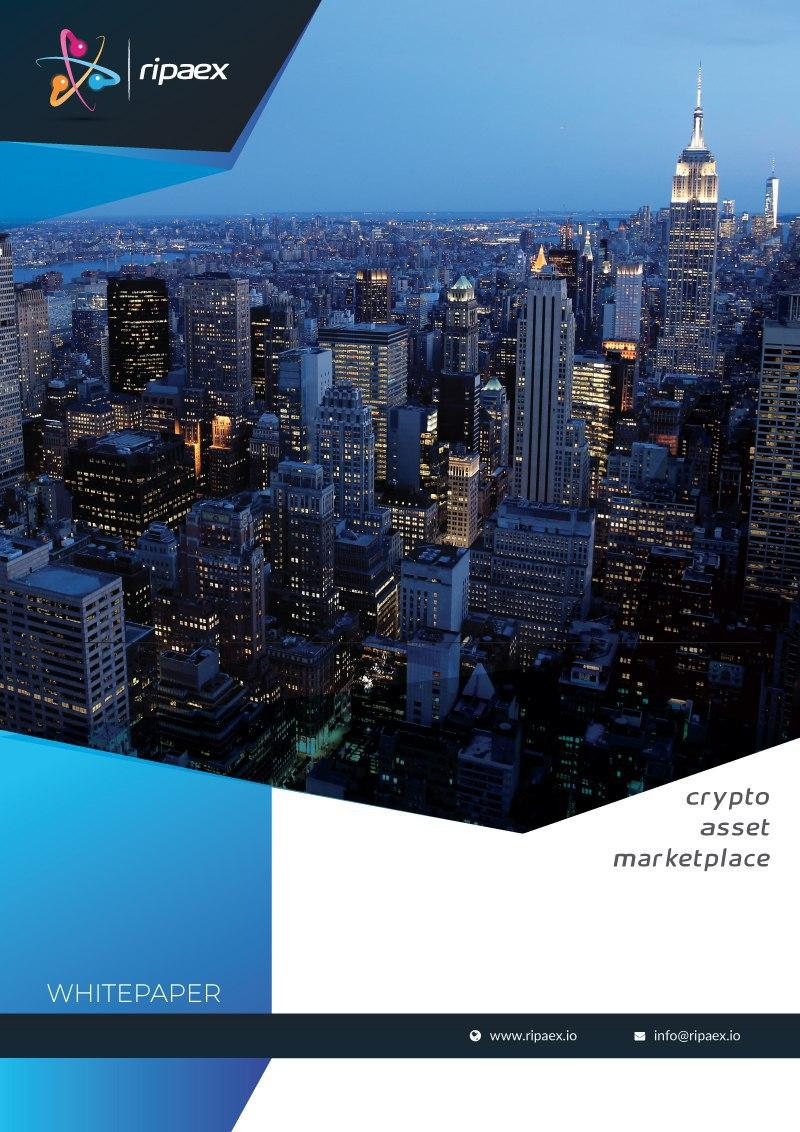
\includegraphics[height=\paperheight]{background}};
\end{tikzpicture}
\endgroup

\newpage

% \begingroup
% \section{Abstract}\index{Abstract}
% \thispagestyle{empty}
% \addcontentsline{toc}{chapter}{\textcolor{trolleygrey}{Abstract}}
\usechapterimagefalse % If you don't want to include a chapter image, use this to toggle images off - it can be enabled later with \usechapterimagetrue
\chapter{Abstract}
\textbf{Ripa Exchange is a hybrid-decentralized exchange with a strong focus on lowering the entry level
of opening new exchanges and giving crypto traders safe and secure trading partners to operate on a daily basis.}\\

The team of Ripa Exchange believes that, despite the recent developments in the world of
cryptocurrencies, it is still expensive to open, manage and build trust on a newly created exchange not
only for the resources need to run a reliable exchange platform but also for the build of the platform 
itself and to find the liquidity necessary to run a profitable business in the first 3-5 year gap.\\

Action is needed and action is needed now. Users are frustrated with unreliable exchanges that run away
with their funds, got hacked or does not sustain the load of a growing industry like this is. Despite
the effort of exchanges managers to offer efficient, reliable, and easy to use platforms to trade entry
prices for building such platforms is in the rage of five-six hundred thousand dollars and that does not 
include personnel cost to give platinum customer support, platform infrastructure and daily expenses for
the business. All of that for then having an decent exchange platform for which you will need to pay an 
external software company to make changes as you request.\\

It is the aim of this project to give you an Open Source, efficient, reliable exchange platform and to
give the needed liquidity\footnote{Thank you to the RLSP (Ripa Liquidity Service Provider) technology} to your newly created 
exchange from day \textbf{one} so you can focus on finding your customers, give platinum support and comply with all the heterogeneous 
laws in the industry. As we want that the customer experience will be the best (the sleekest) as possible while making them safer to trade.\\
\usechapterimagetrue
% \endgroup

%----------------------------------------------------------------------------------------
%	TABLE OF CONTENTS
%----------------------------------------------------------------------------------------

%\usechapterimagefalse % If you don't want to include a chapter image, use this to toggle images off - it can be enabled later with \usechapterimagetrue

\chapterimage{chapter_head_1_Beijing.jpg} % Table of contents heading image
% \addcontentsline{toc}{chapter}{\textcolor{trolleygrey}{Table of Contents}}
\renewcommand*\contentsname{Table of Contents}
\tableofcontents % Print the table of contents itself

% \pagestyle{empty} % No headers

% \cleardoublepage % Forces the first chapter to start on an odd page so it's on the right

% \pagestyle{fancy} % Print headers again

%----------------------------------------------------------------------------------------
%	PART
%----------------------------------------------------------------------------------------


%\part{Part One}

%----------------------------------------------------------------------------------------
%	CHAPTER 2: Introduction
%----------------------------------------------------------------------------------------

\chapterimage{chapter_head_2_London.jpg} % Chapter heading image

\chapter{Introduction}
- The industry of virtual currencies has (a high entry level from a technical point of view for the average user
and) an high entry level from an economical point of view for the average entrepreneur for buying a reliable cryptocurrency 
exchange source code, to hire professional DevOps personnel, to hire customer support operatives, to comply with national and 
international AML/KYC regulations to have liquidity from day one of the exchanges operations. We want to lower this entry level because
\textbf{running an exchange is HARD} and we want you to focus on things that matters not of caveats that the industry require because
you want to start to make business in this industry and you need the source code to do it.

To strengthen that there is the point that starting an exchange require an high level of investments form your venture capital 
and also with that the profit of your exchanges operations are not guaranteed in the first 5 years timespan.

For building a professional exchange services we think that the source code of your exchange and the liquidity to offer to your clients
from day one should be given to you free of charge: no more paying \$150,000.00 to a company just to have a platform that works and for
which you need to pay another \$100,000.00 - 150,000.00 just to brand it and customize as for your needs so you can tide your 
business to a company that may go bankrupt in the future and found you in trouble as you never had the source code of the product
your business rely on.

\textbf{We believe that all of this should be free} and we should offer you the best technology in the market so you can focus on your business
while we focus on building the technology to run your business in an efficient, secure, responsive and productive way. That is why Ripa Exchange 
is focusing on building a network of exchanges focusing on an exchange architecture that is \textit{efficient, secure, UI responsive, compliant and customizable}
so each exchange in the network can rely on solid foundations while customising its single exchange instance for the needs 
the business entity of that particular exchange installation needs.

For reaching that goal we chosen to build our Ripa Liquidity Service Provider technology on top of ARK - a blockchain for consumer adoption - 
which primary focus is increasing consumer adoption for blockchain technologies focusing on two critical areas: \underline{A Fast Secure Core Technology}
and \underline{Practical Services for Real People}. ARK ecosystem is still at its early stage of development: in current implementation 
there is the possibility to run smart contracts natively on the ARK 2.0 blockchain, this will permits this blockchain technology to compete 
with Ethereum from a technological point of view.

The Ripa Founder Team (RFT), as presented on ripaex.io, acts in the name of the Ripa Crew. The RFT is responsible for the proper use of 
funds collected under the Token Exchange Campaign (RIPA - TEC) presented below in this document.

The RFT undertakes that the result of this TEC will be used exclusively for the financing of the \emph{Ripa Exchange} project as explained in this 
whitepaper - which will be made available on the collection platform: tec.ripaex.io - and which should result in the creation of a 
legal entity whose name will be \emph{Ripa Exchange}. The creation of this company is scheduled for the first quarter of 2019.

To this end, RFT intervenes on behalf of \emph{Ripa Exchange, a company in the process of being incorporated}.


%------------------------------------------------

%This statement requires citation \cite{article_key}; this one is more specific \cite[162]{book_key}.

%------------------------------------------------

\section{Key Terminology}\index{Key Terminology}
\begin{description}
	\item[Ripa Exchange]: a FIAT <-> CRYPTO exchange (a cryptocurrency exchange) based on the source code
	of Peatio \cite{peatio}
	\item[Ripa Blockchain]: a DPOS blockchain in which liquidity is exchanged for all the exchanges in the Ripa network
	\item[Ripa Token (XPX)]: a cryptographically secure token exchanged on the Ripa blockchain based on the DPOS protocol
	\item[RIPA]: the DPOS financial ecosystem composed of Ripa Exchange and Ripa Blockchain
	\item[RIPAEX]: the name of the project, project website and hosted domain
    \item[RLSP]: Ripa Liquidity Service Provider, a shared orderbook to exchange orders between exchanges in the same Ripa network
	\item[ARK]: a platform for consumer adoption of blockchain technologies \cite{ark}
	\item[ACES]: Ark Contract Execution Services \cite{aces} provides simple protocols and tools for building a robust 
	blockchain service marketplace based on the ARK SmartBridge technology
    \item[“,” or “.”]: The Anglo-Saxon use of decimal points and commas to represent numbers has
been chosen for the purposes of this document: that is to say that a “.” represents a decimal point, and a “,”
distinguishes between multiples of thousands, millions and billions.
    \end{description}

%Lists are useful to present information in a concise and/or ordered way\footnote{Footnote example...}.

\section{Roadmap}\index{Roadmap}
There are essentially four phases to the RipaEx project:

\begin{description}
	\item[Funding the project: XPX presale and RIPA TEC (WP2)] This phase recognises the existence of interest in this market development
	from across the World concerning the lowering of the entry level for building a cryptocurrency exchange.
	It aims to make the first comprehensive analysis of this state of the art to form the basis of the later project phases and
	build the first working prototype of a centralized exchange based on Peatio. \textbf{Phase ending January 2019}.
	\item[First exchange opening and development of tools and resources (WP3)] The second phase takes the results of the first 
	and develops from them a set of tools and resources which provide concise and comprehensible guidance to market actors in any
	Country. With the first instance of Ripa Exchange running first contacts with other economical players in the industry can be
	done. \textbf{Phase ending June 2019}.
	\item[Development of hybrid-decentralized exchange (WP 4-6)] Using the tools and resources developed in WP3, 
	Work packages 4-6 focus on bringing collected knowledge and tools into practice. The three work packages reflect three major
	focal points (and target groups) within the network of exchange created for establishing successful 
	demonstrations on local scale: incorporations of local Ripa Exchanges (WP4), technical analysis for the 
	Ripa Liquidity Service Provider (WP5), and first MVP of the hybrid decentralized exchange (WP6). The demonstration
    phase forms the heart of the RipaEx action; WP 2 and 3 are focused on providing
    deliverables (e.g. tools) that enable successful and efficient demonstration activities. \textbf{Phase ending January 2020}.
	\item[Dissemination (WP 7/8) and Project Coordination (WP1)] During the full duration of the project, 
	dissemination activities (WP 7/8) are carried out in which results from the individual work packages are disseminated 
	to relevant target groups including project partners, RipaEx supporters, exchanges managers, banking partners as well 
	as relevant target groups. This phase covers a wide range of dissemination techniques, from printed and
    electronic handbooks to workshops and training sessions, ongoing networks, all having the
	ultimate goal of defining a standard for exchanges communication among public and private entities. 
	An overarching work package is concerned with the management of the project from start to finish, ensuring proper coordination, 
	quality assurance and budgetary control (WP1).
\end{description}

\section{RipaEx Partners - RipaEx Governance}\index{RipaEx Partners - RipaEx Governance}
Most of the partners are entrepreneurs in the virtual currency industry, but a research institute 
and Financial Organizations are also represented. The Partners are:
\begin{description}
	\item[Coordinator]: Ripa Exchanges Ltd
	\item[CoBeneficiaries]: 
\end{description}
\subsection{RipaEx Governance}\index{RipaEx Governance}
Governance for the network of exchanges created, development of the source code, owning of the XPX tokens, Ripa Foundation.

\section{Summary}\index{Lists!Summary}
\begin{enumerate}
	\item RipaEx is a project to facilitate the uptake of standards to share liquidity between crypto assets marketplaces. 
	The objective of RipaEx is the promotion of shared source code for wallets and exchanges in the virtual currency industry: 
	It is the aim of this reference document to give in-depth information to prospective exchange developers,
	or exchange managers, to enable correct decision-making and to ensure success for their proposed projects. 
	It seeks to analyse the real potential in the Country of application for a network of cryptocurrency exchanges, 
	and its place in the market.
	\item Crypto assets are an alternative to centralized assets managed by (country-specific) stock exchanges. Although certain
	stock exchanges gives the possibility to their users to verify and manage the assets they own the verification process
	is not always transparent that is the reason because from 2009 \cite{bitcoin} onwards a new types of (community-verifiable) assets 
	have been implemented to give small, medium and big investors complete transparency in the managing of their investments
	assets.
	\item Recent developments at European Union level and worldwide are transforming both how virtual currencies
	are treated and the way ICO (Initial Coin Offering) are legislated. These combined developments 
	have made the use and production of virtual currencies an increasingly favourable prospect. \\
	In October 2015 the European Court of Justice ruled that bitcoin and other cryptocurrencies are exempt from VAT taxation. \\
	In July 2016 the European Commission adopted proposals for legislation to amend the 4th Anti-Money Laundering Directive (4AMLD) that
	will bring virtual currencies exchanged and wallet providers into the EU's anti-money laundering framework \cite{EUAMLCrypto}.\\
	In February 2018 the European Commission launched the EU Blockchain Observatory and Forum \cite{EUBOaF} to highlight key developments 
	of the blockchain technology, promote European actors and reinforce European engagement with multiple stakeholders involved in blockchain activities.
	\item However there is still very little regulation performed on ICOs and only United States of America at the moment has undergone
	a legislation defining ICO tokens as securities. \cite{SECICO}
	\item The results indicate that medium tech savvy from 18 to 45 is the average user of
	virtual currencies although the corporate finance companies are also starting to put 
	virtual currencies schemes inside their portfolio especially since the presentation 
	of the bitcoin futures contract from CME Group Inc. in the stock exchange of Chicago
	last 18th of December 2017.
	\item Total virtual currencies market capitalization has been estimated around 317 B USD\footnote{Coinmarketcap data April 2018}
	and is predicted to grow to 5,000.00 B USD in the next ten years span \cite{cryptoMCTenYears}.
	\item Local authorities are working with National Governments to make sure local exchangers
	in the national territory are complying with national and international AML/KYC regulations.
	Venture capitals and Angel Investors are starting to release financing solutions to start-ups 
	in the Fintech industry all over the world from America to Asia passing through Europe and some 
	Countries are starting state-owned cryptocurrencies schemes to test the exchange of goods \& services
	on those (distributed ledger) technologies \cite{petro}.
	\item The average cost for starting your own crypto asses marketplace is around \$ 150,000.00 only for a running instance of your exchange platform:
	to that you need to add costs to customize the platform before launch and in the future, advertising your new business, running costs for servers,
	network operators, support center operators and legal department to comply with your State of incorporation AML/KYC legislations and general company laws.\\
	\textbf{That is the reason because we think owning the source code of your exchange software is the best way to run a business in this industry}.
	\item The main problems encountered in opening a FIAT <-> CRYPTO marketplace is to find trusted
	banking partners to comply with the many different AML/KYC rule and procedures to exchange virtual currencies
	to FIAT currencies.
	\item Classical types of exchanges operations are: 
		\begin{enumerate}[label*=\arabic*.]
			\item \textbf{one-way exchanges}: in which a centralized application has all the liquidity to offer to its potential users
			\item \textbf{two-way exchanges}: in which a centralized or decentralized platform match the selling requests with the buying requests
			of its users
		\end{enumerate}
		On this a sub-classification is also necessary:
		\begin{enumerate}[label*=\arabic*.]
			\item \textbf{FIAT <-> CRYPTO exchanges}: in which exchanges operations are performed between FIAT\footnote{Traditional central banks owned currencies like EUR, USD, GBP, JPY, others...} 
			currencies and virtual currencies
			\item \textbf{CRYPTO <-> CRYPTO exchanges}: in which exchanges operations are performed only between virtual currencies
		\end{enumerate}
	You can build a matrix based on the four configurations above to build the exchange operation platform of your needs.
	\item The specifications to look when choosing for an exchange platform to run are:
		\begin{enumerate}[label*=\arabic*.]
			\item \textbf{code}: Open Source, Closed Source or hybrid solution
			\item \textbf{modularization}: separation between exchange engine (orders matching engine), UI and user registry
			\item \textbf{UI responsiveness}
			\item \textbf{compliance} with current industry standards
			\item \textbf{customization} of the exchange engine, trading currencies, UI and other aspects of the crypto asset marketplace platform...
			\item \textbf{security} of the funds: saving in cold wallets and hot wallets configurable
			\item \textbf{transparency} of the funds: proof of solvency of the exchange
			\item \textbf{Multi-Accounts}: possibility to user Google, Facebook, Twitter accounts to login into the platform and FIDO Alliance security standards for personal credentials.
		\end{enumerate}	
	\textbf{Those are not only technical decisions to be made but also economical} especially the owning of the source code of your crypto asset
	marketplace platform is fundamental to make future customization of your exchange in an independent way compared to rely on a single
	software house that makes the customizations for you.
	\item Options for finding users for your exchanges operations are: targeted marketing campaigns, innovative features in the industry,
	fee level based on trading quantities, bonuses for first registration and trading quantities, affiliate marketing for paying users to take their friends
	to your exchange.
	\item For setting-up a crypto asset marketplace a project must take into account the following legislation:
		\begin{enumerate}[label*=\arabic*.]
			\item \textbf{AML/KYC}: \textit{Fourth Anti-Money Laundering Directive} if business set up in the European Union \cite{4AMLD} or the AML/KYC reference implementation
			to your crypto asset marketplace Country of incorporation (as an example \textit{Intelligence Reform \& Terrorism Prevention Act of 2004}
			written by FinCEN in the United States of America).\\
			International raccomandations for undergoing AML/CFT verifications are given by the Financial Action Task Force on Money Laundering \cite{FATF}.
			\item \textbf{Payment Licence}: By far the biggest and most arduous task with regards to legitimising the 
			FIAT <-> CRYPTO exchanges operations is obtaining a \textit{PSD Licence} \cite{PSD}. 
			The PSD licence follows Council Directive 2007/64/EC and is applied in each country via its own national laws. 
			Costs of an IPPC licence can vary between \euro XXXX and \euro XXXX, depending on the size of operation.
		\end{enumerate}
	\item The nature of the business under consideration by the Ripa Exchange project (small scale,
	localised FIAT <-> CRYPTO exchanges operations), means that each enterprise likely to have 7 or 8 staff: N.2 developers, 
	N.1 network/security operator, N.1 administrative, N.2 client support operators, N.1 legal and tax advisor. \\
	The turnover of such an enterprise however, because of the high value of the end product, is likely to be more than 
	\euro 350,000 a year and could be several times higher. A business of
	this scale lends itself to the following possible company structures: A simple partnership;
	A limited company; A non-profit company or social enterprise; A worker co-operative.
	Financial Agencies are potential key actors, but the type of business they can set up will
	depend on their legal status which does vary from country to country.
	\item Potential sources of funds for a small-scale biodiesel projects are: Bank Loans; Low
	Interest Loan Schemes; Commercial Credit; Equity financing; Business Angels venture
	capital. Having a robust Business Plan and financial guarantees are essential elements
	for securing funding. The European Investment Fund (EIF) of the EIB, offers support in
	the form of guarantees for SMEs.
	\item The arguments for crypto asset marketplaces are for financial freedom, decentralizing of the value-trasferring operations, and
	owning for real your money. 
	There are other benefits, well documented, such as faster payments, long term gain based on deflactionary economy and prediction of 
	Great Depressions like the one that hit the global economy in 2008. But
	above all, virtual currencies are the only direct competitor to centralized value-transferring operations done by central banks.

	\item There is consensus in the literature that the use of virtual currencies in place of fiat currencies will result in 
	higher financial freedom especially as they fit into the Austrian school of economy \cite{austrianTheory} 
	(TODO: add more on austrian economics school)

	\item Benefits of virtual currencies schemes (TODO: put some numbers)

	\item Securing assets on the blockchains means basically performing three operations
		\begin{enumerate}[label*=\arabic*.]
			\item \textbf{Generating a random private key}
			\item \textbf{Converting the private key generated in (1) into a public key}: a common protocol making this conversion
			in the virtual currencies industry is the ECDSA curve algorithm
			\item \textbf{Converting the public key generated in (2) into a virtual currency address}: common protocols for making this conversion
			are hash functions SHA-256, Base58 encoding, Base32 encoding
		\end{enumerate}
	At this point any value sent to the virtual currency address generated in (3) is secured on the blockchain of choice and accessible
	only from the owner of the relative private key generated in (1).
	\item The two critical factors affecting the cryptocurrency industry are banks concurrence and State banning.
	Although a harmonisation throughout Europe would be beneficial to development of the industry both in terms of 
	taxation and warranty approvals, this is currently not the case. Each country has its specific legislation and tax
	regime for all exchanges operations involving FIAT money, and State banning is going to completely liberalization 
	of this activiteis like European Union to complete banning and imprisonment of operators in this industry like Bangladesh
	\cite{bitcoinLegality}. 

	\item The asiatic countries of South Korea, China and Japan are the leader in the field of cryptocurrencies for number of 
	transactions for over 9 years with a proactive approach and favourable tax regime. At the beginning of 2017 in Japan bitcoin
	has been declared legal tender but China has recently declared illegal token sale and exchanges and local cryptocurrencies
	marketplaces are closing down.
	\item Any assessment of your local market should include: number of potential users to reach, 
	type of exchange to incorporate (FIAT <-> CRYTPO or CRYPTO <-> CRYPTO), type of virtual currencies protocol 
	to integrate (POW, DPOS, Masternodes, others...), types of services to offer (exchange only, advanced trading tools,
	payment processor, others...), if FIAT <-> CRYPTO exchange number of FIAT payments processors to accept (PayPal, OKPay,
	MoneyPolo, others...), number of others exchanges in your region.

	\item there are a number of options for dealing with Warranty/Customer protection issues: 
	creating consumer pressure by making clear to the end users that the possession of the private keys of their
	virtual currency addresses make \textbf{liable} for any loss of the private keys meaning nobody can help
	them recovering their funds if the their private keys are lost. Creating consumer pressure to not leave funds
	on exchanges ("\textit{Be Your own Bank!!}"), making them choose the licesed exchanges in the market. 
	\item While it is very expensive to insure money exchanges operations and money transmitting operations, 
	examples of customer protections in the industry are: Kraken platform which is offering Mt. Gox users partial refund
	of their losts, NEO community giving refund to the users involved in the BitGrail hacking, Ethereum supporters
	giving The DAO investors partial refunds, other hacking cases...

	\item Recommendations for all/for law compliance: if you inted to incorporate a FIAT <-> CRYPTO exchange you should
	focus from the first instance on law complicance by studing the AML/KYC laws of the country of incorporation and
	finding bank partners to work with. Local financial Authoriy can help to comply with rules \% regulations and 
	local cryptocurrencies foundations can help you to tune your exchanges operations to perform targeted
	operations based on the customers interests in the country of incorporation.
	Promote cryptocurrency-friendly users in the area of interest.
\end{enumerate}


%----------------------------------------------------------------------------------------
%	CHAPTER 3: Ripa Exchange
%----------------------------------------------------------------------------------------

\chapterimage{chapter_head_3_Singapore.jpg} % Chapter heading image

\chapter{The Ripa Exchange}

\section{Theorems}\index{Theorems}

This is an example of theorems.

\subsection{Several equations}\index{Theorems!Several Equations}
This is a theorem consisting of several equations.

\begin{theorem}[Name of the theorem]
	In $E=\mathbb{R}^n$ all norms are equivalent. It has the properties:
	\begin{align}
		 & \big| ||\mathbf{x}|| - ||\mathbf{y}|| \big|\leq || \mathbf{x}- \mathbf{y}||                            \\
		 & ||\sum_{i=1}^n\mathbf{x}_i||\leq \sum_{i=1}^n||\mathbf{x}_i||\quad\text{where $n$ is a finite integer}
	\end{align}
\end{theorem}

\subsection{Single Line}\index{Theorems!Single Line}
This is a theorem consisting of just one line.

\begin{theorem}
	A set $\mathcal{D}(G)$ in dense in $L^2(G)$, $|\cdot|_0$.
\end{theorem}

%------------------------------------------------

\section{Definitions}\index{Definitions}

This is an example of a definition. A definition could be mathematical or it could define a concept.

\begin{definition}[Definition name]
	Given a vector space $E$, a norm on $E$ is an application, denoted $||\cdot||$, $E$ in $\mathbb{R}^+=[0,+\infty[$ such that:
	\begin{align}
		 & ||\mathbf{x}||=0\ \Rightarrow\ \mathbf{x}=\mathbf{0}        \\
		 & ||\lambda \mathbf{x}||=|\lambda|\cdot ||\mathbf{x}||        \\
		 & ||\mathbf{x}+\mathbf{y}||\leq ||\mathbf{x}||+||\mathbf{y}||
	\end{align}
\end{definition}

%------------------------------------------------

\section{Notations}\index{Notations}

\begin{notation}
	Given an open subset $G$ of $\mathbb{R}^n$, the set of functions $\varphi$ are:
	\begin{enumerate}
		\item Bounded support $G$;
		\item Infinitely differentiable;
	\end{enumerate}
	a vector space is denoted by $\mathcal{D}(G)$.
\end{notation}

%------------------------------------------------

\section{Remarks}\index{Remarks}

This is an example of a remark.

\begin{remark}
	The concepts presented here are now in conventional employment in mathematics. Vector spaces are taken over the field $\mathbb{K}=\mathbb{R}$, however, established properties are easily extended to $\mathbb{K}=\mathbb{C}$.
\end{remark}

%------------------------------------------------

\section{Corollaries}\index{Corollaries}

This is an example of a corollary.

\begin{corollary}[Corollary name]
	The concepts presented here are now in conventional employment in mathematics. Vector spaces are taken over the field $\mathbb{K}=\mathbb{R}$, however, established properties are easily extended to $\mathbb{K}=\mathbb{C}$.
\end{corollary}

%------------------------------------------------

\section{Propositions}\index{Propositions}

This is an example of propositions.

\subsection{Several equations}\index{Propositions!Several Equations}

\begin{proposition}[Proposition name]
	It has the properties:
	\begin{align}
		 & \big| ||\mathbf{x}|| - ||\mathbf{y}|| \big|\leq || \mathbf{x}- \mathbf{y}||                            \\
		 & ||\sum_{i=1}^n\mathbf{x}_i||\leq \sum_{i=1}^n||\mathbf{x}_i||\quad\text{where $n$ is a finite integer}
	\end{align}
\end{proposition}

\subsection{Single Line}\index{Propositions!Single Line}

\begin{proposition}
	Let $f,g\in L^2(G)$; if $\forall \varphi\in\mathcal{D}(G)$, $(f,\varphi)_0=(g,\varphi)_0$ then $f = g$.
\end{proposition}

%------------------------------------------------

\section{Examples}\index{Examples}

This is an example of examples.

\subsection{Equation and Text}\index{Examples!Equation and Text}

\begin{example}
	Let $G=\{x\in\mathbb{R}^2:|x|<3\}$ and denoted by: $x^0=(1,1)$; consider the function:
	\begin{equation}
		f(x)=\left\{\begin{aligned}    & \mathrm{e}^{|x|} &  & \text{si $|x-x^0|\leq 1/2$} \\
			 & 0                &  & \text{si $|x-x^0|> 1/2$}\end{aligned}\right.
	\end{equation}
	The function $f$ has bounded support, we can take $A=\{x\in\mathbb{R}^2:|x-x^0|\leq 1/2+\epsilon\}$ for all $\epsilon\in\intoo{0}{5/2-\sqrt{2}}$.
\end{example}

\subsection{Paragraph of Text}\index{Examples!Paragraph of Text}

\begin{example}[Example name]
	\lipsum[2]
\end{example}

%------------------------------------------------

\section{Exercises}\index{Exercises}

This is an example of an exercise.

\begin{exercise}
	This is a good place to ask a question to test learning progress or further cement ideas into students' minds.
\end{exercise}

%------------------------------------------------

\section{Problems}\index{Problems}

\begin{problem}
What is the average airspeed velocity of an unladen swallow?
\end{problem}

%------------------------------------------------

\section{Vocabulary}\index{Vocabulary}

Define a word to improve a students' vocabulary.

\begin{vocabulary}[Word]
	Definition of word.
\end{vocabulary}

%----------------------------------------------------------------------------------------
%	PART
%----------------------------------------------------------------------------------------

%\part{Part Two}

%----------------------------------------------------------------------------------------
%	CHAPTER 4: Ripa Blockchain
%----------------------------------------------------------------------------------------

\chapterimage{chapter_head_4_Dubai.jpg} % Chapter heading image

\chapter{The Ripa Blockchain}

\section{Table}\index{Table}

\begin{table}[h]
	\centering
	\begin{tabular}{l l l}
		\toprule
		\textbf{Treatments} & \textbf{Response 1} & \textbf{Response 2} \\
		\midrule
		Treatment 1         & 0.0003262           & 0.562               \\
		Treatment 2         & 0.0015681           & 0.910               \\
		Treatment 3         & 0.0009271           & 0.296               \\
		\bottomrule
	\end{tabular}
	\caption{Table caption}
\end{table}

%------------------------------------------------

\section{Figure}\index{Figure}

\begin{figure}[h]
	\centering
\includegraphics[scale=0.5]{placeholder}
	\caption{Figure caption}
\end{figure}


%----------------------------------------------------------------------------------------
%	CHAPTER 5: Token Sale
%----------------------------------------------------------------------------------------

\chapterimage{chapter_head_5_Tokyo.jpg} % Chapter heading image

\chapter{Token Sale}

\section{Table}\index{Table}

\begin{table}[h]
	\centering
	\begin{tabular}{l l l}
		\toprule
		\textbf{Treatments} & \textbf{Response 1} & \textbf{Response 2} \\
		\midrule
		Treatment 1         & 0.0003262           & 0.562               \\
		Treatment 2         & 0.0015681           & 0.910               \\
		Treatment 3         & 0.0009271           & 0.296               \\
		\bottomrule
	\end{tabular}
	\caption{Table caption}
\end{table}

%------------------------------------------------

\section{Figure}\index{Figure}

\begin{figure}[h]
	\centering
\includegraphics[scale=0.5]{placeholder}
	\caption{Figure caption}
\end{figure}

%----------------------------------------------------------------------------------------
%	CHAPTER 6: Conclusion
%----------------------------------------------------------------------------------------

\chapterimage{chapter_head_6_Frankfurt.jpg} % Chapter heading image

\chapter{Conclusion}


%----------------------------------------------------------------------------------------
%	CHAPTER 7: Legal
%----------------------------------------------------------------------------------------

\chapterimage{chapter_head_7_LosAngeles.jpg} % Chapter heading image

\chapter{Legal}

%----------------------------------------------------------------------------------------
%	BIBLIOGRAPHY
%----------------------------------------------------------------------------------------

\chapterimage{chapter_head_8_KualaLumpur.jpg} % Chapter heading image

\addcontentsline{toc}{chapter}{\textcolor{trolleygrey}{References}}
\nocite{*}
\printbibliography[title={References}]
%------------------------------------------------


%----------------------------------------------------------------------------------------
%	COPYRIGHT PAGE
%----------------------------------------------------------------------------------------

\newpage
~\vfill
\thispagestyle{empty}

\noindent Copyright \copyright\ 2018 Ripa Founder Team\\ % Copyright notice

\noindent \textsc{Published by Ripa Founder Team}\\ % Publisher

\noindent \textsc{www.ripaex.io}\\ % URL

\noindent Licensed under the MIT License (the ``License''). You may not use this file except in compliance with the License. You may obtain a copy of the License at \url{https://opensource.org/licenses/MIT}. Unless required by applicable law or agreed to in writing, software distributed under the License is distributed on an \textsc{``as is'' basis, without warranties or conditions of any kind}, either express or implied. See the License for the specific language governing permissions and limitations under the License.\\ % License information

\noindent \textit{First printing, March 2018} % Printing/edition date

\end{document}
